% !TeX document-id = {2870843d-1baa-4f6a-bd0a-a5c796104a32}
% !BIB TS-program = biber
% !TeX encoding = UTF-8
% TU Delft beamer template

\documentclass[aspectratio=43]{beamer}
\usepackage[english]{babel}
\usepackage{csquotes}
\usepackage{calc}
\usepackage[absolute,overlay]{textpos}
\usepackage{graphicx}
\usepackage{subfig}
\usepackage{mathtools}
\usepackage{amsfonts}
\usepackage{amsthm}
\usepackage{comment}
\usepackage{siunitx}
\usepackage{MnSymbol,wasysym}
\usepackage{array}
\usepackage{qrcode}
\useoutertheme[subsection=false]{miniframes}

\setbeamertemplate{navigation symbols}{} % remove navigation symbols
\mode<presentation>{\usetheme[verticalbar=false]{tud}}

% BIB SETTINGS
\usepackage[
    backend=biber,
    giveninits=true,
    maxnames=30,
    maxcitenames=20,
    uniquename=init,
    url=false,
    style=authoryear,
]{biblatex}
\addbibresource{bibfile.bib}
\setlength\bibitemsep{0.3cm} % space between entries in the reference list
\renewcommand{\bibfont}{\normalfont\scriptsize}
\setbeamerfont{footnote}{size=\tiny}
\renewcommand{\cite}[1]{\footnote<.->[frame]{\fullcite{#1}}}
\setlength{\TPHorizModule}{\paperwidth}
\setlength{\TPVertModule}{\paperheight}

\newcommand{\absimage}[4][0.5,0.5]{%
	\begin{textblock}{#3}%width
		[#1]% alignment anchor within image (centered by default)
		(#2)% position on the page (origin is top left)
		\includegraphics[width=#3\paperwidth]{#4}%
\end{textblock}}

\newcommand{\mininomen}[2][1]{{\let\thefootnote\relax%
	\footnotetext{\begin{tabular}{*{#1}{@{\!}>{\centering\arraybackslash}p{1em}@{\;}p{\textwidth/#1-2em}}}%
	#2\end{tabular}}}}

\title[]{Localización de landmarks cefalométricos por medio de técnicas de few-shot learning y análisis de redes convolucionales}
\institute[]{\textbf{Tutores}: Pablo Mesejo Santiago, Javier Merí de la Maza \and Universidad de Granada, España}
\author{Alejandro Borrego Megías}
\date{27 de Noviembre de 2022}



%%%%%%%%%%%%% EMPIEZA LA PRESENTACION %%%%%%%%%%%%%
\begin{document}

{
\setbeamertemplate{footline}{\usebeamertemplate*{minimal footline}}
\frame{\titlepage}
}

% Parte de Matemáticas
\part{Análisis de Redes convolucionales}

%INDICE
\begin{frame}{Índice Primera Parte}
  \textcolor{tudCyan}{\textbf{Análisis de redes convolucionales}}
  \medskip
  \tableofcontents[part=1]
\end{frame}

% DIAPOSITIVA ANTES DE CADA SECCION
% \AtBeginSection[ ]
% {
% \begin{frame}{Índice Primera Parte}
%     \tableofcontents[currentsection]
% \end{frame}
% }

%INTRODUCCION
\section{Introducción}
  \begin{frame}[fragile]{Redes Neuronales Convolucionales}
    \begin{itemize}
      \item Buen rendimiento, comprobable empíricamente.
      \item Vía de estudio abierta en lo que se refiere a
      la modelización matemática y la justificación teórica de estos resultados.
    \end{itemize}

    propiedades: 

    \begin{figure}
      \centering
      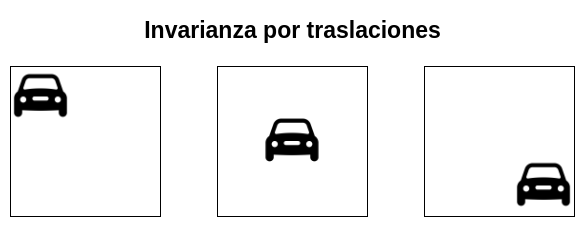
\includegraphics[width=0.4\textwidth]{imgs/translation_invariance.png}
    \end{figure}

    \begin{figure}
      \centering
      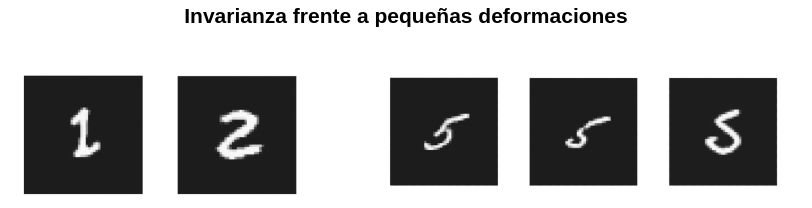
\includegraphics[width=0.7\textwidth]{imgs/Deformaciones.png}
    \end{figure}
  \end{frame}

  \begin{frame}{Invarianza por traslaciones}
    Trabajamos sobre el espacio de funciones $L^2(\mathbb{R}^d)$.

    \begin{block}{Definición de traslación}
       Sea $f\in L^2(\mathbb{R}^d)$, $L_cf(x)=f(x-c)$ es la traslación de $f$ por $c \in \mathbb{R}^d$.
    \end{block}

    \begin{block}{Invarianza por traslaciones de un operador $\Phi$}
      Decimos que un operador $\Phi$ sobre  $L^2(\mathbb{R}^d)$, es invariante por traslaciones si $\Phi(L_cf)=\Phi(f)$ para todo $f \in L^2(\mathbb{R}^d)$ y para todo $c \in \mathbb{R}^d$.
   \end{block}
  \end{frame}

  \begin{frame}[t]{Invarianza frente a pequeñas deformaciones}
    \textcolor{tudCyan}{\textit{Deformación $\implies$ Difeomorfismo}}

    \textcolor{tudCyan}{\textit{Deformaciones pequeñas $\implies$ Difeomorfismos cercanos a traslaciones}}  

    \begin{block}{Definición}
      Denotemos $L_{\tau} f(x)=f(x-\tau(x))$ como la acción del difeomorfismo $1-\tau$ sobre $f$.

      Donde $\tau$ es el campo de desplazamiento. 
    \end{block}

  \end{frame}

  \begin{frame}{Invarianza frente a pequeñas deformaciones}
    \textcolor{tudCyan}{\textbf{\centering Invarianza frente a pequeñas deformaciones \\ \centering $\Downarrow$ \\ \centering Lipschitz-continuidad frente a la acción de difeomorfismos}}  

    \begin{block}{Invarianza frente a pequeñas deformaciones de un operador $\Phi$}
      \begin{equation*}
        \| \Phi(f)-\Phi(L_{\tau}f)\|\leq C\|f\|(\|\nabla\tau\|_{\infty} + \|H \tau\|_\infty).
      \end{equation*}
      Con $f\in L^2(\mathbb{R}^d)$ y $C>0$.
    \end{block}
  \end{frame}


  \begin{frame}{Objetivo}
    \centering \LARGE \textcolor{tudCyan}{\textbf{Encontrar un operador $\Phi$ que cumpla lo anterior y modelice una red convolucional}}
  \end{frame}

\section{Modelización}

\begin{frame}{Módulo de la transformada de Fourier}
  $$\Phi(f)=|\widehat{f}| \;\; f\in L^2(\mathbb{R}^2)$$

  Con este operador observamos que: 
  \begin{itemize}
    \item Es invariante por traslaciones.
    \item No es Lipschitz continuo frente a pequeñas deformaciones.
  \end{itemize}

  Debemos buscar otro operador.
\end{frame}

\begin{frame}{Alternativa: Ondeletas}
  Usaremos ondeletas madre del tipo: 

  \begin{equation*}
    \psi(x)=e^{i\eta x} \Theta(x)
  \end{equation*}
  donde $\Theta(x)$ es una función real con soporte en una bola de baja frecuencia en $x=0$, cuyo radio es del orden de $\pi$.

  \begin{block}{Escalado y rotación de ondeleta madre}
    Una ondeleta madre escalada por un factor $2^{j}$ con $j \in \mathbb{Z}$ y rotada por $r \in G$ siendo $G$ el grupo finito de rotaciones, se escribe: 
    $$\psi_{2^j r}(x)=2^{j} \psi(2^j r^{-1} x).$$
  \end{block}
\end{frame}

\begin{frame}{La transformada de Littlewood-Paley}
  Con esta generamos la siguiente base ortonormal de ondeletas: 
  \begin{equation*}
    \lbrace \psi_\lambda (x) \rbrace_{\lambda= 2^j r \in 2^\mathbb{Z} \times G}
  \end{equation*}

  \begin{block}{Transformada de Littlewood-Paley}
    \begin{equation*}
      \forall x \in  \mathbb{R}^d \;\; W[\lambda]f(x)= f \ast \psi_\lambda(x)=\int f(u)\psi_\lambda(x-u) du .
    \end{equation*}
    donde $\lambda \in 2^j r \in 2^\mathbb{Z} \times G$
  \end{block}

  El operador $W[\lambda]f=f\ast \psi_\lambda$ es Lipschitz-continuo bajo la acción de difeomorfismos para $f \in L^2(\mathbb{R}^d)$ fijo. 

  \medskip

  \textcolor{tudCyan}{¿Pero invariante a traslaciones?}
\end{frame}

\begin{frame}{Problema: La escala}
  \begin{figure}
    \centering
    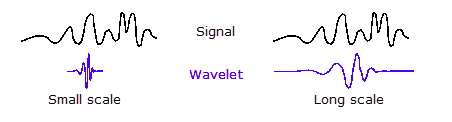
\includegraphics[width=0.8\textwidth]{imgs/Relacion_escala_frecuencia.png}
  \end{figure}
  Fijada una escala $2^J \; \; J\in \mathbb{Z}$, se establece un umbral tal que solo se mantienen las ondeletas de escala $2^j > 2^{-J}$.
\end{frame}

\begin{frame}{Problema: La escala}
  Surge la necesidad de promediar las frecuencias no cubiertas por el factor de escala fijado:

  \begin{equation*}
    A_Jf=f \ast \phi_ {2^J} \; \; \text{con} \quad \; \phi_ {2^J}(x)=2^{-J} \phi(2^{-J}x).
  \end{equation*}

  Así, los coeficientes obtenidos, fijada una escala son:

  $$W_J f=\lbrace A_Jf,(W[\lambda]f)_{\lambda \in \Lambda_J} \rbrace$$ 

  con $\Lambda_J=\lbrace \lambda=2^jr:\;r\in G^{+}, \; 2^j>2^{-J}\rbrace$.

  \begin{itemize}
    \item Bajo hipótesis no muy restrictivas sobre las ondeletas y $\phi$ los coeficientes cumplen $\| W_J \|=1$.
  \end{itemize}
\end{frame}

\begin{frame}{Restricciones}
  Tranajaremos con funciones reales.
  \begin{itemize}
    \item $W_J$ es unitario. 
    \item $\widehat{\phi}(\omega)$ es real y simétrica, por lo que $\phi$ también lo será. 
    \item Las derivadas de $\phi$ pertenecen a $L^1(\mathbb{R}^d)$.
  \end{itemize}
\end{frame}

\begin{frame}{Propagador de dispersión}

  \begin{alertblock}{Condición para coeficientes I.T.}
    Si $U[\lambda]$ es un operador definido en $L^2(\mathbb{R}^d)$, no necesariamente lineal pero que conmuta con traslaciones, entonces $\int_{\mathbb{R}^d} U[\lambda]f(x)dx$ es invariante a traslaciones si es finito.
  \end{alertblock}
  \medskip
  Pero como $\int_{\mathbb{R}^d} \psi(x)dx=0 \implies \int_{\mathbb{R}^d} f \ast \psi(x) dx=0$. 
\end{frame}

\begin{frame}{Propagador de dispersión}
  Para obtener coeficientes invariantes por traslaciones. 
  $$U[\lambda]f= \textcolor{red}{M[\lambda]} W[\lambda]$$

  \medskip

  El operador más sencillo que garantiza coeficientes invariantes por traslaciones y Lipschitz-continuidad frente a difeomorfismos es:

  \begin{block}{Definición del operador $U[\lambda]$}
    $$U[\lambda]f=M[\lambda]W[\lambda]f=|f \ast \psi_\lambda|=\left | \int_{\mathbb{R}^d} f(u)\psi_\lambda(x-u) du \right|$$
  \end{block}
\end{frame}


\begin{frame}{Propagador de dispersión}

  \begin{block}{Camino}
    Una secuencia ordenada $p=(\lambda_1,\lambda_2, \ldots , \lambda_m)$ con $\lambda_k \in \Lambda_\infty=2^{\mathbb{Z}} \times G^{+} $ se denomina \textbf{camino}. Al camino vacío se le denota por $p=\emptyset$. 
  \end{block}

  Así, sobre un camino $p$ definimos el \textbf{propagador de dispersión} como: 

  $$  U[p]f=U[\lambda_m] \ldots U[\lambda_2]U[\lambda_1]f=\left| |f \ast \psi_{\lambda_1} | \ast \psi_{\lambda_2} | \ldots | \ast \psi_{\lambda_m} \right|
  $$

  \medskip

  Además:

  $$ \int_{\mathbb{R}^d} U[p]f(x)dx < \infty $$
\end{frame}


% \begin{frame}{Operador de dispersión}
%   \begin{alertblock}{Operador de dispersión}
%     Sea $\mathcal{P}_\infty$ el conjunto de todos los caminos finitos. La transformada de dispersión de $f \in L^1(\mathbb{R}^d)$ se define para cualquier camino $p \in \mathcal{P}_\infty$ como:
%     \begin{equation*}
%       \overline{S}f(p)=\int_{\mathbb{R}^d}U[p]f(x)dx
%     \end{equation*}
%   \end{alertblock}

%   Siendo $\overline{S}f(p)$ invariante a traslaciones para un $f$ fijo.
% \end{frame}

\begin{frame}{Operador de ventana}
  \begin{block}{Definición operador de ventana}
    Sea $J \in \mathbb{Z}$ y $\mathcal{P}_J$ el conjunto de caminos finitos $p=(\lambda_1,\lambda_2,...,\lambda_m)$ con $\lambda_k \in \Lambda_J$ y $|\lambda_k|=2^{k}>2^{-J}$. Una ventana de transformada de dispersión se define para todo $p \in \mathcal{P}_J$ por
    \begin{equation*}
      S_J[p]f(x)=U[p]f \ast \phi_{2^J}(x)=\int_{\mathbb{R}^d}U[p]f(u)\phi_{2^J}(x-u)du.
    \end{equation*}
    \begin{equation*}
      S_J[p]f(x)=\left| |f \ast \psi_{\lambda_1} | \ast \psi_{\lambda_2} | \ldots | \ast \psi_{\lambda_m} \right| \ast \phi_{2^J}(x).
    \end{equation*}
  \end{block}
\end{frame}

\begin{frame}{Diferencias y Similitudes con una red convolucional}
  \textbf{\textcolor{tudCyan}{Similitudes:}}
  \begin{itemize}
    \item Cascada de convoluciones (operador $W[\lambda]$).
    \item Capas de \textit{pooling} (operador $M[\lambda]$ y $\phi_{2^J}$).
    \item Si $p$ tiene longitud $m$: $S_J[p]f(x)$ equivale al resultado de la capa $m$ de la red.
  \end{itemize}

  \textbf{\textcolor{tudCyan}{Diferencias:}}
  \begin{itemize}
    \item Los pesos no se aprenden.
  \end{itemize}
\end{frame}

\section{Invarianza por traslaciones}

\begin{frame}{Ondeletas admisibles}
  
  \begin{block}{ondeletas admisibles}
    Una ondeleta de dispersión se dice que es admisible si existe $\eta \in \mathbb{R}^d$ y una función $\rho \geq 0$, con $|\widehat{\rho}(\omega)| \leq |\widehat{\phi}(2\omega)|$ y $\widehat{\rho}(0)=1$, tal que la función: 

    \begin{equation*}\label{eq::1.6}
      \widehat{\Psi}(\omega)=|\widehat{\rho}(\omega - \eta)|^2 - \sum_{k=1}^{+\infty} k(1-|\widehat{\rho}(2^{-k}(\omega - \eta))|^2)
    \end{equation*}
      
    \noindent satisface: 
    \begin{equation*} \label{eq::1.7}
      \alpha= \inf_{1\leq|w|\leq2} \sum_{j=-\infty}^{\infty} \sum_{r\in G} \widehat{\Psi} (2^{-j}r^{-1}\omega)|\widehat{\psi}(2^{-j}r^{-1}\omega)|^2>0.
    \end{equation*}
  \end{block}


\end{frame}

\begin{frame}{No-expansividad y conservación de la norma}

  \begin{alertblock}{No-expansividad}
    \noindent Para $f,h \in L^2(\mathbb{R}^d)$ y $J\in \mathbb{Z}$ se cumple

    \begin{equation*} \label{eq::1.10}
      || S_{J+1} [\mathcal{P}_{J+1}]f- S_{J+1}[\mathcal{P}_{J+1}]h || \leq ||S_J[\mathcal{P}_J]f - S_J[\mathcal{P}_J]h ||. 
    \end{equation*}
  \end{alertblock}

  \begin{alertblock}{Conservación de la norma}
    Si las ondeletas son admisibles, entonces para toda $f\in L^2(\mathbb{R}^d)$ se tiene que
    \begin{equation*}  
      \lim_{m\rightarrow\infty} \sum_{n=m}^{\infty} \|S_J[\Lambda_J^n]f\|^2=0
    \end{equation*}
    y
    \begin{equation*}
      \|S_J[\mathcal{P}_J]f\|=\|f\|.
    \end{equation*}
  \end{alertblock}
\end{frame}

\begin{frame}{Invarianza por traslaciones}
  \begin{alertblock}{Invarianza por traslaciones}
    Para ondeletas de dispersión admisibles se tiene que 
    $$\forall f \in L^2(\mathbb{R}^d), \; \forall c\in \mathbb{R}^d \;\;\; \lim_{J\rightarrow \infty}||S_J[\mathcal{P}_J] f-S_J[\mathcal{P}_J] L_cf||=0.$$
  \end{alertblock}
\end{frame}

% Parte de Informática
\part{Localización de landmarks cefalométricos por medio de técnicas de few-shot learning}

\begin{frame}{Índice Segunda Parte}
  \textcolor{tudCyan}{\textbf{Localización de landmarks cefalométricos por medio de técnicas de few-shot learning}}
  \medskip
  \tableofcontents[part=2]
\end{frame}

% Current section
% \AtBeginSection[ ]
% {
% \begin{frame}{Índice Segunda Parte}
%     \tableofcontents[currentsection]
% \end{frame}
% }

\section{Definición del Problema}


\begin{frame}{Landmarks cefalométricos}
  \begin{itemize}
    \item Puntos de referencia que \textbf{definen la morfología del cráneo}.
    \item \textbf{Correspondencia} directa \textbf{cráneo-cara}.
    \item Se emplean en \textbf{Antropología forense}.
  \end{itemize}
  \begin{figure}
    \centering
    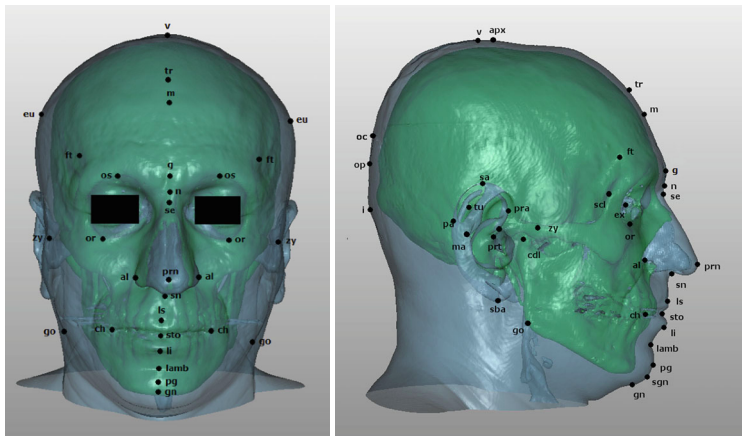
\includegraphics[width=0.45\textwidth]{imgs/marcado_landmarks.png}
    \caption{Imagen extraída de \cite{damas2020handbook}}
  \end{figure}
\end{frame}

\begin{frame}{Landmarks faciales}
  \begin{itemize}
    \item Puntos de referencia \textbf{marcados sobre la cara}.
    \item \textbf{No guardan relación} con la morfología del cráneo.
    \item Se emplean para \textbf{reconocimiento facial}.
  \end{itemize}

  \begin{figure}
    \centering
    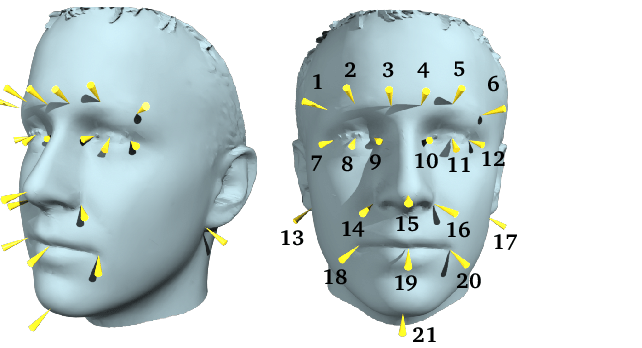
\includegraphics[width=0.6\textwidth]{imgs/aflw.png}
    \caption{Landmarks marcados en AFLW \cite{AFLW}}
  \end{figure}

\end{frame}

\begin{frame}[t]{Base de datos}
  \begin{columns}[onlytextwidth]
    \begin{column}{.5\textwidth}
      \begin{itemize}
        \item 167 imágenes \textbf{\textit{in-the-wild}}.
        \item Imágenes a \textbf{color y escala de grises}.
        \item \textbf{30 landmarks} a predecir.
      \end{itemize}  
      % square filling the column
      % place an image
      % horizontal position = 73%
      % vertical position = 45%
      % width = 40% of page
      \absimage{.3, .7}{.45}{imgs/EjemplosBD.png}
    \end{column}
    \begin{column}{.5\textwidth}
      % square filling the column
      % place an image
      % horizontal position = 73%
      % vertical position = 45%
      % width = 40% of page
      \absimage{.75, .49}{.19}{imgs/vertical.png}
    \end{column}
  \end{columns}
\end{frame}


\begin{frame}{Objetivos}
  \begin{enumerate}
    \item Revisión del \textbf{estado del arte}.
    \item Investigación sobre los \textbf{Autoencoders} y \textbf{redes adversarias} existentes.
    \item Estudio y \textbf{preprocesamiento} de la base de datos.
    \item Estudio \textbf{experimental} usando diversos modelos que derivan del framework principal.
  \end{enumerate}
\end{frame}

\section{Fundamentos Teóricos}

% \begin{frame}{Redes Neuronales Convolucionales}
%   \begin{figure}
%     \centering
%     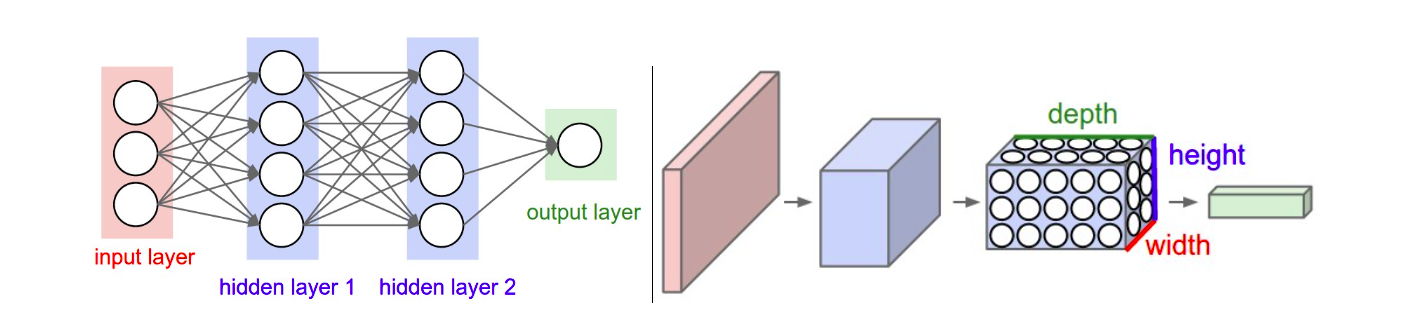
\includegraphics[width=0.99\textwidth]{imgs/ArquitecturaRedNeuronal.png}
%     \caption{Imagen extraída de \cite{StanfordCourse}.}
%   \end{figure}
% \end{frame}

\begin{frame}{Arquitectura de una red neuronal convolucional}
  \begin{figure}
    \centering
    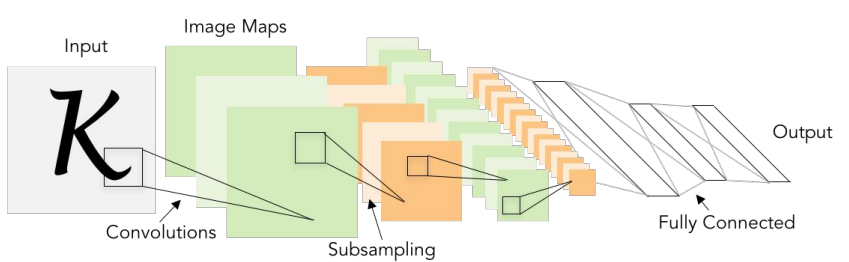
\includegraphics[width=0.99\textwidth]{imgs/ArquitecuraGeneral.png}
    \caption{Imagen extraída de \cite{StanfordCourse}.}
  \end{figure}
\end{frame}

\begin{frame}{Capas Convolucionales}
  \begin{columns}[onlytextwidth]
    \begin{column}{.5\textwidth}
       \textbf{Características:}
      \begin{itemize}
        \item Operación de convolución.
        \item Menor número de pesos.
        \item Mayor profundidad de red.
      \end{itemize}
      Imágenes extraída de \cite{StanfordCourse}.
    \end{column}
    \begin{column}{.5\textwidth}
      \absimage{.75, .30}{.50}{imgs/mapa_activacion.png}
      \absimage{.75, .65}{.45}{imgs/sucesion_conv_layer.png}
    \end{column}
  \end{columns}
\end{frame}

\begin{frame}{Capa de Pooling}
  \begin{figure}
    \centering
    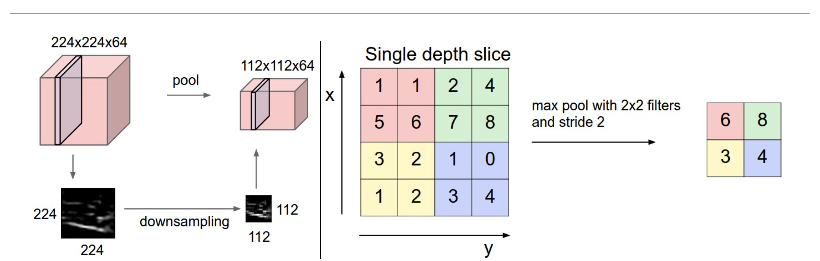
\includegraphics[width=0.99\textwidth]{imgs/pooling.png}
    \caption{Imagen extraída de \cite{StanfordCourse}.}
  \end{figure}
\end{frame}

\begin{frame}{Capa totalmente conectada}
  \begin{figure}
    \centering
    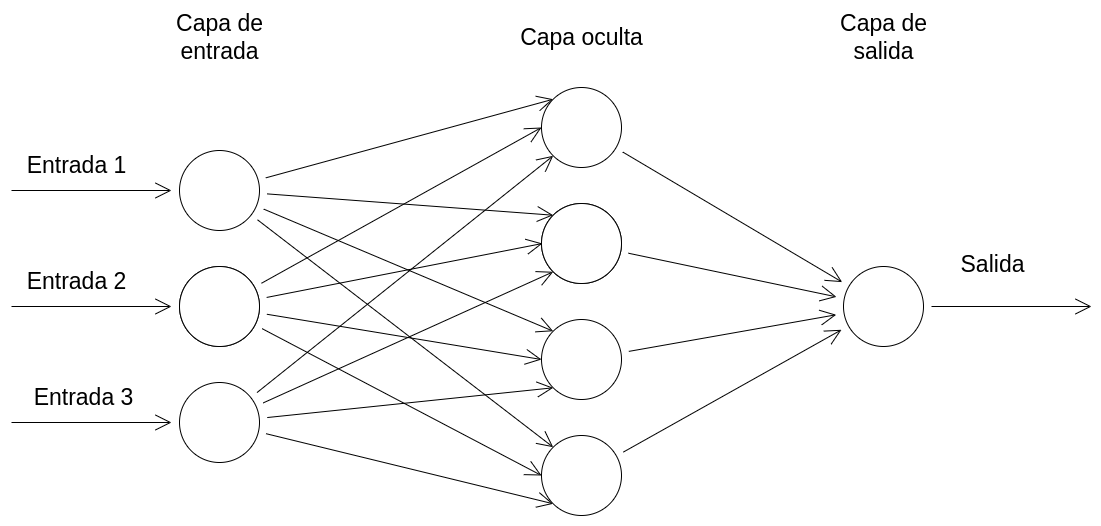
\includegraphics[width=0.99\textwidth]{imgs/single_hidden_layer.png}
  \end{figure}
\end{frame}

% \begin{frame}{Autoencoders}
%   \begin{figure}
%     \centering
%     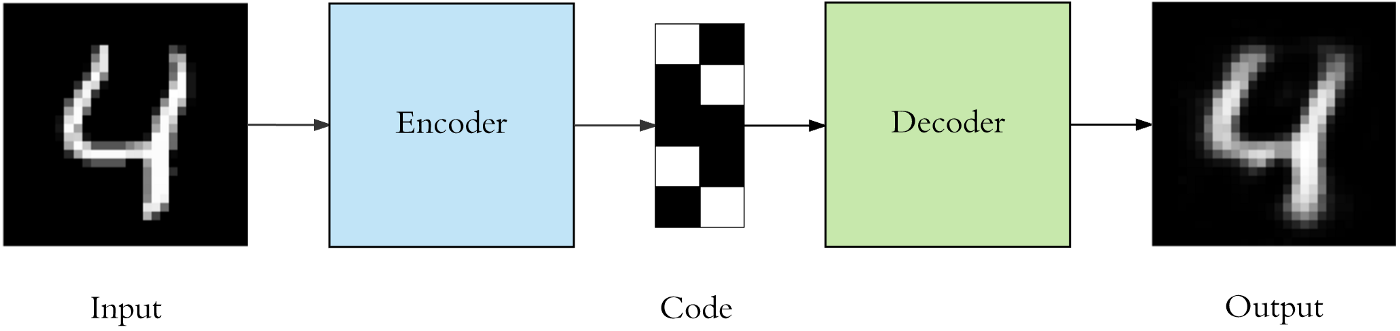
\includegraphics[width=0.99\textwidth]{imgs/Autoencoder.png}
%     \caption{Imagen extraída de \cite{autoencoders2017}.}
%   \end{figure}
% \end{frame}

% \begin{frame}{Variational Autoencoder (VAE)}
%   \begin{columns}[onlytextwidth]
%     \begin{column}{.5\textwidth}
%       \absimage{.25, .50}{.5}{imgs/VAE_1.png}
%       Imágenes extraída de \cite{VAE}.
%     \end{column}
%     \begin{column}{.5\textwidth}
%       \absimage{.75, .53}{.5}{imgs/VAE_2.png}
%     \end{column}
%   \end{columns}
% \end{frame}

% \begin{frame}{Generative Adversarial Network(GAN)}
%   \begin{figure}
%     \centering
%     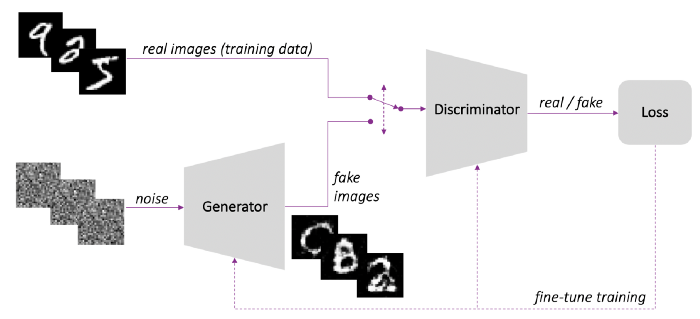
\includegraphics[width=0.99\textwidth]{imgs/GAN.png}
%     \caption{Imagen extraída de \cite{GAN}.}
%   \end{figure}
% \end{frame}

\begin{frame}{Adversarial Autoencoder (AAE)}
  \begin{figure}
    \centering
    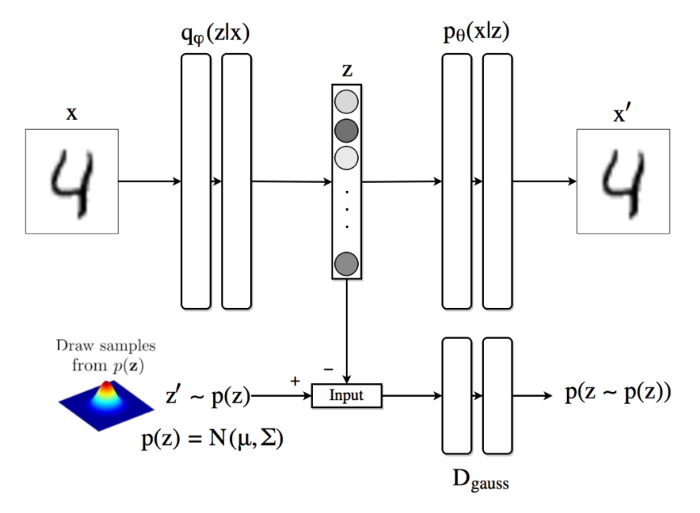
\includegraphics[width=0.6\textwidth]{imgs/AAE.png}
    \caption{Imagen extraída de \cite{AAE}.}
  \end{figure}
\end{frame}

\section{Estado del arte}

\begin{frame}[t]{Búsqueda Scopus}

  \begin{columns}[onlytextwidth]
    \begin{column}{.5\textwidth}
      \textbf{Landmarks faciales}:
      \begin{itemize}
        \item Gran número de artículos.
        \item Deep learning.
      \end{itemize} 
      % square filling the column
      % place an image
      % horizontal position = 73%
      % vertical position = 45%
      % width = 40% of page
      \absimage{.25, .60}{.45}{imgs/Scopus_1.png}
    \end{column}
    \begin{column}{.5\textwidth}
      \textbf{Landmarks cefalométricos}:
      \begin{itemize}
        \item Escasa literatura. \item Gran variedad de enfoques.
      \end{itemize}
      % square filling the column
      % place an image
      % horizontal position = 73%
      % vertical position = 45%
      % width = 40% of page
      \absimage{.75, .60}{.45}{imgs/Scopus_2.png}
    \end{column}
  \end{columns}
\end{frame}

\begin{frame}[t]{Taxonomía}
  \begin{itemize}
    \item Encontramos 13 artículos en total.
    \item Sólo 4 relacionados con el marcado de landmarks cefalométricos.
    \item Emplean diversas técnicas de \textbf{visión por computador} y \textbf{aprendizaje automático}.
  \end{itemize}
  \begin{figure}
    \centering
    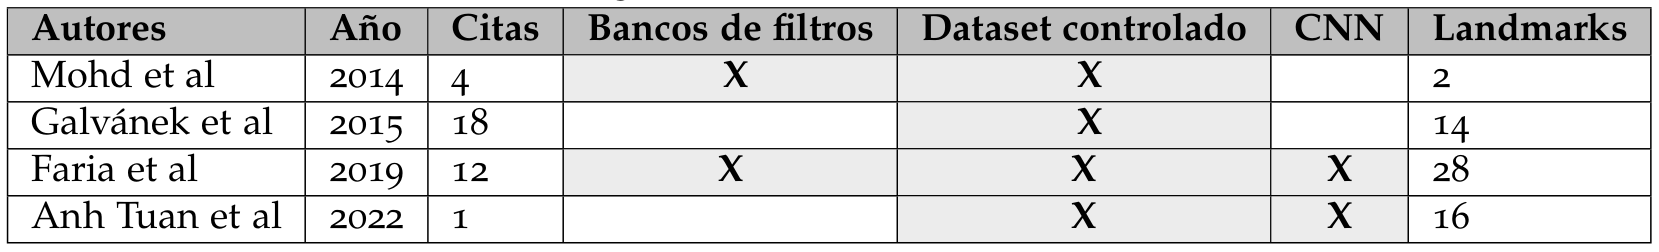
\includegraphics[width=0.99\textwidth]{imgs/taxonomia.png}
  \end{figure}
\end{frame}

\section{Experimentos}

\begin{frame}[t]{3FabRec}
  \begin{figure}
    \centering
    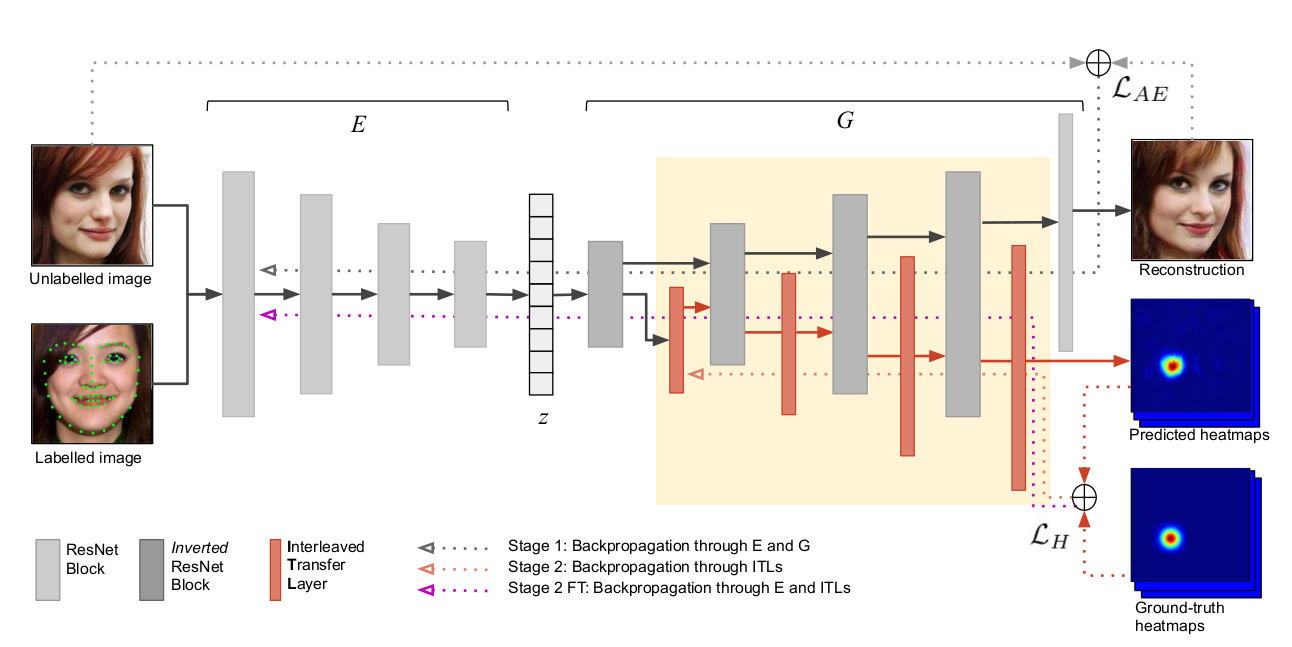
\includegraphics[width=0.85\textwidth]{imgs/3fabrec_arquitectura.png}
    \caption{Imagen extraída de \cite{browatzki20203fabrec}.}
  \end{figure}
\end{frame}

% \begin{frame}{3FabRec}
%   \begin{block}{Función de pérdida parte no supervisada}
%     \begin{align*}
%       \min_{E,G} \max_{D_z,D_x} & \mathcal{L}_{AE}(E,G,D_z,D_x) = \\
%       & \lambda_{rec} \mathcal{L}_{rec}(E,G) + \lambda_{cs}\mathcal{L}_{cs}(E,G) \\
%       & + \lambda_{enc}\mathcal{L}_{enc}(E,D_z)+ \lambda_{adv} \mathcal{L}_{adv}(E,G,D_x)
%     \end{align*}
%   \end{block}
%   \begin{block}{Función de pérdida parte supervisada}
%     \begin{equation*}
%       \mathcal{L}_H(ITL) = \mathbb{E}_{x ~ p(x)} \left[ \| H-ITL(a)\|_2 \right]
%     \end{equation*}
%   \end{block}
% \end{frame}

\begin{frame}{3FabRec}
  \textcolor{tudCyan}{\textbf{Bases de datos de la parte no supervisada}}
  \begin{itemize}
    \item VGGFace2 + AffectNet
    \item En total $2.1$ millones de imágenes.
  \end{itemize}
  \textcolor{tudCyan}{\textbf{Bases de datos de la parte supervisada}}
  \begin{itemize}
    \item 300W $= 3.148$ imágenes.
    \item AFLW $= 24.386$ imágenes.
    \item WFLW $= 10.000$ imágenes.
  \end{itemize}
\end{frame}

\begin{frame}[t]{Preprocesamiento}
  \begin{columns}[onlytextwidth]
    \begin{column}{.65\textwidth}
      \begin{itemize}
        \item Realizamos \textbf{detección + \textit{cropping}} de caras en las imágenes del dataset.
        \item Empleamos red auxiliar \textbf{Facenet}.
        \item \textbf{Problema}: Algunos landmarks quedan fuera del \textit{bounding box}. Se necesita un \textbf{reajuste}.
      \end{itemize} 
      % square filling the column
      % place an image
      % horizontal position = 73%
      % vertical position = 45%
      % width = 40% of page
      \absimage{.3, .7}{.45}{imgs/bb_1.png}
    \end{column}
    \begin{column}{.5\textwidth}
      % square filling the column
      % place an image
      % horizontal position = 73%
      % vertical position = 45%
      % width = 40% of page
      \absimage{.75, .49}{.25}{imgs/bb_2.png}
    \end{column}
  \end{columns}
\end{frame}

\begin{frame}[t]{Reajuste 3FabRec}
  \begin{itemize}
      \item Bounding box cuadrado de lado \textbf{$\max(h,w)$}.
      \item Ampliación uniforme por el factor \textbf{$\frac{crop\_size+margin}{crop\_size}$}.
      \item Reescalado a \textbf{tamaño $256 \times 256$}.
      \item \textbf{Problema}: Vertex suele quedar fuera.
  \end{itemize}

  \absimage{0.6, 0.7}{0.6}{imgs/bounding_box_3fabrec.png}
\end{frame}

\begin{frame}[t]{Partición de los datos}
  Se dividen los datos en entrenamiento y test: 
  \begin{itemize}
      \item \textbf{131} imágenes para entrenamiento ($80\%$). Usaremos \textbf{cross-validation 5 fold}.
      \item \textbf{32} imágenes para test ($20\%$).
      \item Durante el preprocesamiento descartamos $4$ imágenes.
  \end{itemize}

  \absimage{0.5, 0.7}{0.8}{imgs/Particion_Datos.png}
\end{frame}

\begin{frame}[t]{Experimentos}
  \begin{itemize}
    \item \small \textbf{Modelo Base}: entrenamiento ITLs $\rightarrow$ \textbf{Adam}
    \item \small \textbf{Ajuste fino del Encoder}: entrenamiento ITLs + Encoder $\rightarrow$ \textbf{Adam}
    \item \small \textbf{Ajuste fino del Decoder}: entrenamiento ITLs + Decoder $\rightarrow$ \textbf{Adam}
    \item \small \textbf{Data Augmentation}: entrenamiento ITLs con técnicas de Data Augmentation $\rightarrow$ \textbf{Adam}
  \end{itemize}

  \absimage{0.5, 0.7}{0.85}{imgs/EsquemaModelos.png}
\end{frame}

\begin{frame}[t]{Validación de los modelos}
  \textbf{Cross-Validation 5-fold}.
  \begin{figure}
    \centering
    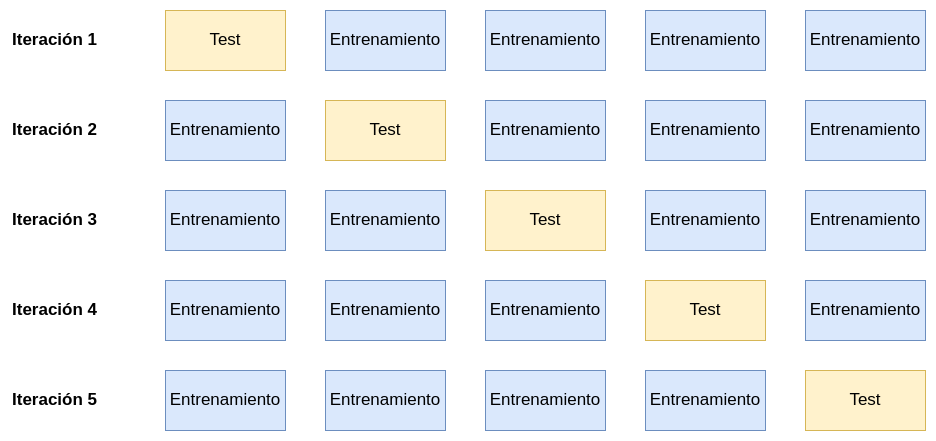
\includegraphics[width=0.99\textwidth]{imgs/5-fold-cv.png}
  \end{figure}

  \absimage{0.87, 0.18}{0.15}{imgs/entrenamiento.png}
\end{frame}

\begin{frame}[t]{Métricas empleadas}
  \normalsize \textbf{Métricas entrenamiento}
    \begin{itemize}
      \item \small MSE:
          \small \begin{equation*}
            MSE = \frac{1}{N} \sum_{i=1}^{N} (y_i - \widehat{y}_i)^2
          \end{equation*}
    \end{itemize}

    \normalsize \textbf{Métricas Validación}
    \begin{itemize}
      \item \small Error de reconstrucción:
        \small \begin{equation*}
          Reconstruction \; Loss = \frac{\sum_{i=1}^n |p_i -q_i|}{N}
        \end{equation*}
      \item \small NME:
          \small \begin{equation*}
          NME=\frac{\sqrt{\sum_{i=1}^{n}(p_{i,1} -q_{i,1})^2+ (p_{i,2} -q_{i,2})^2}}{N}
        \end{equation*}
      \item SSIM:
          \small\begin{equation*}
            cs(x,y)=\frac{1}{|w|} \sum{c(x_w,y_w)s(x_w,y_w)}_w
          \end{equation*}
    \end{itemize}
    \absimage{0.75, 0.18}{0.15}{imgs/entrenamiento.png}
    \absimage{0.87, 0.18}{0.10}{imgs/test.png}
\end{frame}

\begin{frame}[t]{Análisis Cuantitativo}
  \begin{columns}[onlytextwidth]
    \begin{column}{.5\textwidth}
      % square filling the column
      % place an image
      % horizontal position = 73%
      % vertical position = 45%
      % width = 40% of page
      Para cada imagen: 
      \begin{itemize}
        \item NME medio.
        \item Error de reconstrucción medio.
      \end{itemize}

      Se concatenan las salidas de \textbf{cross validation}:
      \absimage{.25, .67}{.45}{imgs/boxplot_sumarize.png}
    \end{column}
    \begin{column}{.5\textwidth}
      Media por landmark de las predicciones de \textbf{cross validation}:
      % square filling the column
      % place an image
      % horizontal position = 73%
      % vertical position = 45%
      % width = 40% of page
      \begin{itemize}
        \item a
        \item a
        \item a
        \item a
      \end{itemize}
      \absimage{.74, .59}{.47}{imgs/tabla_landmarks.png}
    \end{column}
  \end{columns}
\end{frame}


\begin{frame}{Análisis Cualitativo: Modelo Data Augmentation}
  \begin{figure}
    \centering
    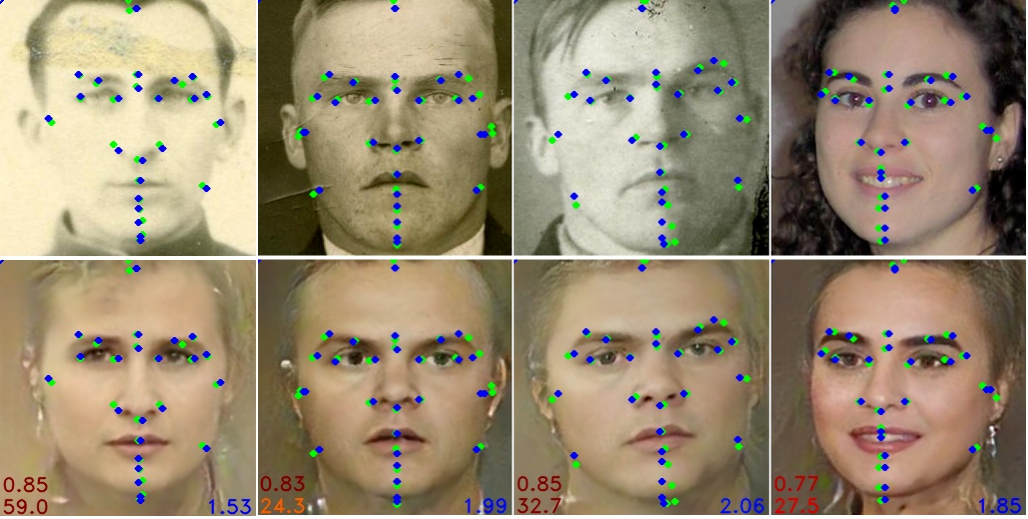
\includegraphics[width=0.99\textwidth]{imgs/image_basemodel.png}
  \end{figure}
\end{frame}

\begin{frame}[t]{Elección de modelo $\rightarrow$ Data Augmentation}

  \begin{columns}[onlytextwidth]
    \begin{column}{.65\textwidth}
      \begin{itemize}
        \item Entrenamos el modelo final con \textbf{todo} el conjunto de entrenamiento.
        \item No hay \textbf{overfitting}.
      \end{itemize}
      \absimage{.30, .60}{.5}{imgs/image_finalmodel.png}
    \end{column}
    \begin{column}{.35\textwidth}
      \absimage{.77, .60}{.45}{imgs/curvas_FinalModel.png}
    \end{column}
  \end{columns}
\end{frame}

\begin{frame}{Comparativa HF-Resnet}

  \begin{columns}[onlytextwidth]
    \begin{column}{.4\textwidth}
      \normalsize \textbf{Diferencias:}
      \begin{itemize}
        \item \scriptsize \textbf{Preprocesamiento}: mismo dataset + 99 modelos $3D$ de caras neutrales.
        \item \scriptsize \textbf{Métricas: }
            \begin{equation*}
              RMSE(y,\widehat{y})= \sqrt{\frac{1}{N} \sum_{i=1}^{N} (y_i-\widehat{y}_i)^2}
            \end{equation*}
      \end{itemize}
      \absimage{.25, .75}{.45}{imgs/tanle_comparativa1.png}
    \end{column}
    \begin{column}{.6\textwidth}
      \absimage{.74, .50}{.5}{imgs/table_comparativa2.png}
    \end{column}
  \end{columns}
\end{frame}

\begin{frame}{Comparativa HF-Resnet}
  \begin{columns}[onlytextwidth]
    \begin{column}{.4\textwidth}
      \begin{itemize}
        \item \textbf{Mejora} generalizada en el marcado.
        \item \textbf{Reducción} de la distancia euclídea media.
        \item \textbf{Mejora} el rendimiento en imágenes complicadas.
      \end{itemize}
    \end{column}
    \begin{column}{.6\textwidth}
      \absimage{.74, .50}{.5}{imgs/compativa_cualitativa.png}
    \end{column}
  \end{columns}
\end{frame}

\section{Conclusiones}

\begin{frame}[t]{Conclusiones}
  \normalsize \textbf{Todos los objetivos cumplidos}
  \begin{enumerate}
    \item \small Investigación + comparación con el estado del arte.
    \item \small Estudio sobre los Autoencoders y redes adversarias.
    \item \small Estudio de errores y preprocesamiento de los dato.
    \item \small Estudio experimental.
  \end{enumerate}

  \medskip

  \normalsize Además, se han logrado otros \textbf{objetivos adicionales}:
  \begin{itemize}
    \item \small Entrenar 3FabRec con landmarks faltantes.
    \item \small Método robusto con few-shot learning.
  \end{itemize}
\end{frame}

\end{document}

